\chapter{Background} % Main chapter title

\label{Chapter 2} % For referencing the chapter elsewhere, use \ref{Chapter1} 
\lhead{Chapter 2. \emph{Background}}

%\section{Chapter2}
\par Planning is among the oldest fields of Artificial Intelligence: it was introduced in the 60s when researchers began considering automated reasoning about actions and changes. The goal of planning is, given a set of actions that describe transitions
between states, to find a plan, i.e. a series of actions to go from an initial state to a specific goal. Such AI planners are used to solve real world problems by reasoning
on a model of the world. It has many applications in Robotics \cite{shin1986dynamic}, Logistics ~\cite{crainic2009models}.
\section{Classical and linear planning}
STRIPS \cite{fikes1972strips} is the first major AI planner. It considers domain knowledge, i.e. a representation of the real world, as a triple: $\ D = (S,A,\gamma), $ with S a set of states, A a set of actions and $\ \gamma: S \times A  \leftarrow S,$ a transition function that maps an initial state and action to the resulting state after performing the action. STRIPS assumes that the actions in the model are deterministic and discrete in time. Each state $\ s \in S $ is a conjunction of positive literals. The world is monotonous (i.e. non-represented literals are false in the state). Each action $\ a \in A $ is of the for $\ A (P, AL, DL) $ with : 
\begin{itemize}
	\item[-] A the action symbol composed by a set of terms (e.g. $\ move(X,Y,Z) $ to represent the action that moves object X from location Y to location Z);
	\item[-] P is the precondition of the action, i.e. a conjunction of positive literals that must be true before the execution of the action;
	\item[-] AD and DL define respectively the add list and the delete list. The former is 	a set of positive literals added to the current state after the action execution 	and the later represents the positive literals removed from the state after the action execution.
\end{itemize}
\par A planning problem is defined as a triple $\ P = <D, si, sg> $ with D is the domain knowledge,$\ si \in S $ the initial state and $\ sg \in S $ the goal state. A solution to P is a plan $\ \pi $, i.e. a sequence of actions $\ a1,..., an \in An $ such that $\ \gamma (Si, \pi) \leftarrow Sg $ (starting from the initial state, the plan leads to the goal state).


\par Several methods exist to solve a STRIPS planning problem. It has been proved \cite{bylander1994computational} that solving a planning problem in STRIPS is \emph{PSPACE} complete. Several heuristics have been developed to find acceptable solutions (closed to the optimal plan in number of steps) in a reasonable time. The initial STRIPS mean-end planner relied on a simple backward chaining search in the
state space. In the 90s, most research focused on searching the plan-space (e.g. \cite{russell2009artificial}). More recent approach such as GRAPHPLAN \cite{blum1997fast} and O-plan \cite{currie1991plan} propose to convert the planning problem to a different structure (e.g. a graph) for better performance.
STRIPS was the foundation of several later works such as PDDL \cite{mcdermott1998pddl}, etc and there still exists an active research field to find better (and faster) planning algorithms.

\section{HTN planning}
 To work properly, the planner requires that the STRIPS problem is provided with a complete model of the domain knowledge, i.e. that the STRIPS representation corresponds to the real world situation. This modeling requires significant knowledge-engineering effort: one of the major difficulties with STRIPS is that all actions are at the same atomic level. As the considered problems become more and more complex, describing all these actions independently turns out to be an impossible task. This is on of the main reasons why new models have been proposed. Hierarchical Task Networks (HTNs) are probably the most commonly used model for planning since the 2000's
\subsection{Overview of HTN}
\par A HTN or Hierarchical Task Network can be thought as AND/OR tree structure (see Figure \ref{HTN tree representation}) where the root node expresses the task to be achieved. Tasks (T) and recipes (R) are alternatives nodes at each level in the tree.

\par Tasks nodes are OR nodes whose children are recipes that can be used to decompose the respective task into more primitive subtasks. Recipes nodes are AND nodes because the children of the recipe are a set of partially or fully ordered tasks resulting from using a recipe to decompose a task, all of which must be performed
when applying the recipe to decompose a task. Non-leaf node tasks represent compound tasks that need to be decomposed by a recipe and the leaf nodes are primitive tasks that can be directly executed. Each node has a set of zero or more modeling specification depending on the HTN modeling. These modeling specifications are pre-conditions, post-conditions and applicability conditions.

\begin{itemize}
	\item Applicability condition: the modeling specification of recipe's nodes which helps the HTN choosing the appropriate decomposition if there is more than	one.
\end{itemize}
The task nodes haves two types of modeling specifications:
\begin{itemize}
	\item Precondition: Specify when a task can be executed, so no task will start until all of its preconditions are satisfied.
	\item Postcondition: Specify when a task execution success or fails, in fact a task execution is considered as complete when its post-conditions are satisfied.
\end{itemize}
\subsection{HTN formalism}
We start the HTN formalism by the presentation of HTN compound namely tasks and recipes.
\subsubsection{Task formalism}
Tasks are expressions of the form $\ T (PC, EC) $ where $T$ is a symbol defining the task name. $ PC $is the preconditions and $ EC$ is postcondition modeled as set of literals. 
\begin{figure}[h]
	\centering
	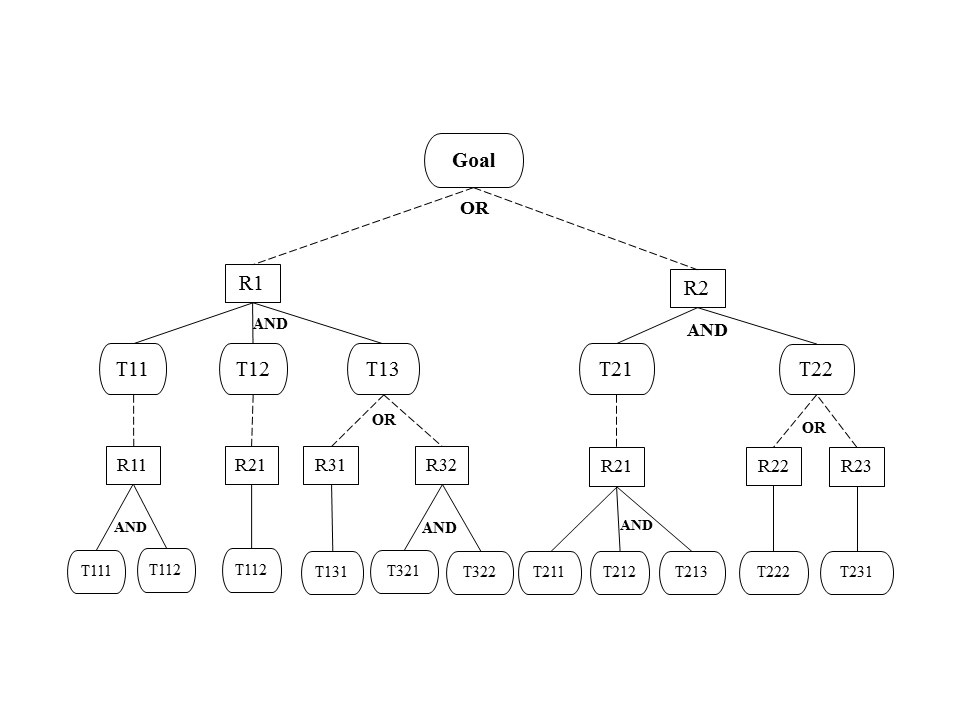
\includegraphics[width=\textwidth]{Pictures/htn1.png}
	\caption{\label{HTN tree representation} HTN tree representation}
\end{figure}


We denote two types of tasks; compound task or non-primitive task and primitive task or action. For example figure \ref{HTN example representation} represents a compound task Move (Obj, Room1, Room2, Door) which is decomposed into three primitive tasks $\{Pick-up (Obj), Walk (Room1, Room2, Door), Put-down(Obj)\}$.

\begin{figure}[h]
	\centering
	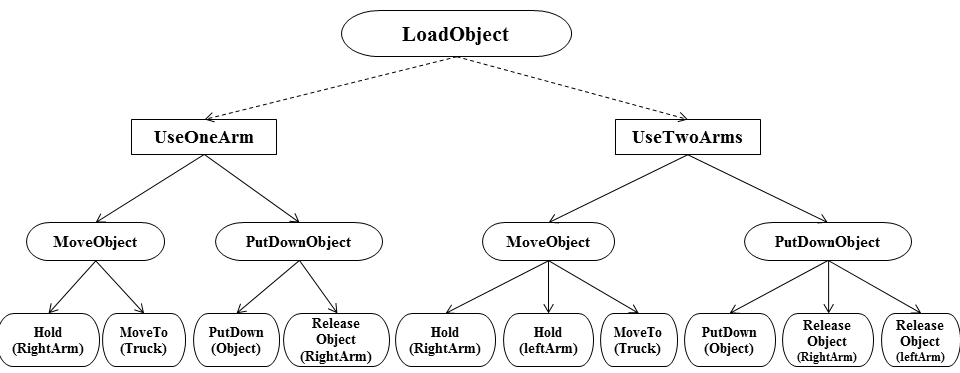
\includegraphics[width=\textwidth]{Pictures/example.png}
	\caption{\label{HTN example representation} HTN example representation}
\end{figure}


\subsubsection{HTN Recipe formalism}
An HTN recipe is used for decomposing compound tasks and has the form of a triple $\ R = (N, T, H)$ where $N$ is the name of the recipe which is unique such that no two recipes can have the same name. $T$ is a non-primitive task performed with this recipe and $H$ is a task network containing the set of subtasks of $T$, describing one way of performing the task T.


Using the HTN components formalism, we present now the domain knowledge and the HTN problem planning.

\par The Domain knowledge $D$ is a list of all the recipes in the HTN needed to decompose the HTN tasks. $\ D= [R1,. . . , Rn].$ Thus an HTN is a tree defined as a tuple $\ M =<T,D> $ where $T$ is the task network composed by all the tasks of the HTN and $D$ is the domain knowledge.

\par The planning problem $P$ is defined as a tree-tuple $\ P =< I, M, G>$ where $\ I$ is the initial state, $M$ is the domain problem defined by the HTN tree and $G$ is the goal task to achieve. $G$ belongs to the tasks of $M$ and the precondition of $G$ is true in $I$. The problem is to find a plan that solves $P$. HTN planning works by expanding tasks and resolving conflicts iteratively, until a conflict-free plan can be found that consists only of primitive tasks.

\par Planning proceeds using task decomposition that starts from the initial goal task $G$, expands this task using a corresponding recipe $R$, and breaks down the goal into sequence of simpler subtasks. This process is applied recursively until the planner reaches a sequence of fully ordered primitive tasks that can make a goal successful. Thus, the solution of the planning problem $P$ is a plan $\ \pi = [a1,.., an]$ is a sequence of primitive tasks $\ ai \in M$ , and $\ i \in [1,n].$

\par The HTN planners are becoming popular in different domains where several systems were developed these recent years such as SHOP \cite{nau1999shop}, SIPE \cite{wilkins1988practical} or NOAH \cite{sacerdoti1975structure}.

\par General purpose of planning as STRIPS and HTN relies on a complete model of the domain knowledge, that means if the model is not complete then, the planner won't be able to plan. This approach of planning is named \emph{Declarative representation}. Such representation of HTN requires a full modeling of HTN domain knowledge. Each
task in the HTN has at least one modeling specification that allows reasoning in planning. Despite the completeness of this representation, modeling such domain require significant knowledge-engineering effort if it is not impossible.

\section{Reactive HTNs}
Declarative approaches for planning attempt to predict the future. The planning is made in off-line phase that start from initial state to search for logical future states to reach a final goal state, using for that the modeling specifications in the domain knowledge. Once the plan is generated, the execution phase is launched in the environment.
\par In contrast with this approach, reactive HTNs propose an approach with no planning phase to predict the future states at all. Instead, they compute just the next task to perform in every instant. Moreover, because of the complexity of modeling a domain knowledge, reactive HTNs run through a hand-authored HTN with a procedural definition of the modeling specifications. Procedural definition of the domain knowledge means that the planner cannot reason about theses conditions, the conditions are script code (example JavaScript)  that can only be executed or evaluated in the current state.

\par The solution of a planning problem is to find a path through the HTN using recipe selection. Starting from the initial state and the goal task, The HTN incrementally generates a sequence of sub-goals by choosing recipes for decomposing tasks. The recipe is selected by the applicability condition at the state where this last can be evaluated. The modeling specifications are evaluated in the current state, if it returns the values true the HTN consider it as valid and continue the exploration of the HTN. However if the evaluation of any specification fails (returns false), the
HTN execution fails and we say that the HTN reaches a dead end. This situation is considered as hard failure. 

The execution is considered as complete if primitive tasks that make the goal successful are reached. Reactive HTN are becoming very popular in the field of controlling complex artificial intelligent systems exist performing in dynamic environment such as Dialog with the Disco system \cite{rich2009building} and RavenClaw \cite{bohus2003ravenclaw}.

\section{Plan execution, breakdown and recovery}
The declarative planners introduced before return a plan $\ \pi $ composed of a sequence of primitive tasks (actions), which is passed to the controller for the execution phase. The execution starts from the initial state and has to achieve the execution
of all the actions of the plan to reach the goal state. The execution of a STRIPS action is valid if its preconditions match subsets of the current observed world state immediately before the action is executed. The effects the executed action are added to the resulting state and the deleted effects are removed from it.

\par The HTN execution takes the STRIPS execution one step further by introducing the postcondition checks. As STRIPS primitive task (action) is applicable if its preconditions are valid in the current state of the world, in addition, the execution of the primitive task is considered as succeed only if its postconditions are part from the resulting state. Thus, the plan is a solution to a planning problem if it matches a subset of the current world state immediately after the last action in the plan is executed.

\par As the environment is dynamic, the controller monitors the environment at each execution step in order to prevent a breakdown. A breakdown occurs if any deviation from the steps defined in the constructed plan is detected, such deviation makes the executed plan invalid and the execution of plan stops. The breakdown
is identified if the world changes in an unexpected way that causes the execution failure of an action. The failure can be caused by one of these situations:
\begin{itemize}
	\item First, the action preconditions are no longer satisfied in the current state. For example, a robot that plans to walk from room1 to room2 through door1, arriving at door1 the wind blows and the door1 became close, this unexpected change invalidate the precondition of the action that is the door must be open.
	\item Second, the executed action leads to unexpected consequences, in this case the postconditions of the action are not satisfied.
\end{itemize}
%
\section{The problem}

Systems presented above need to plan, a complete definition of the domain knowledge which represent the real world faithfully. However,the dynamic definition of the environment in real problems implies unexpected changes that planner must predict and handle. For example, representing cooking problem such in Figure \ref{Cooking model example} involve representing all the actions and devices used. In addition, the model must contain tasks that can handle each change in the environment. For example, when modeling the cook task which involve heat the oven, if an electrical failure happens, then the planner has to react and restores electricity. However,  constructing such complete logical (declarative) model of real and complex problems that run in dynamic environment requires significant knowledge-engineering effort nearly impossible.  Thus, the domain knowledge is  incomplete which may lead the planner to face breakdowns. 
 \begin{figure}[h]
 	\centering
 	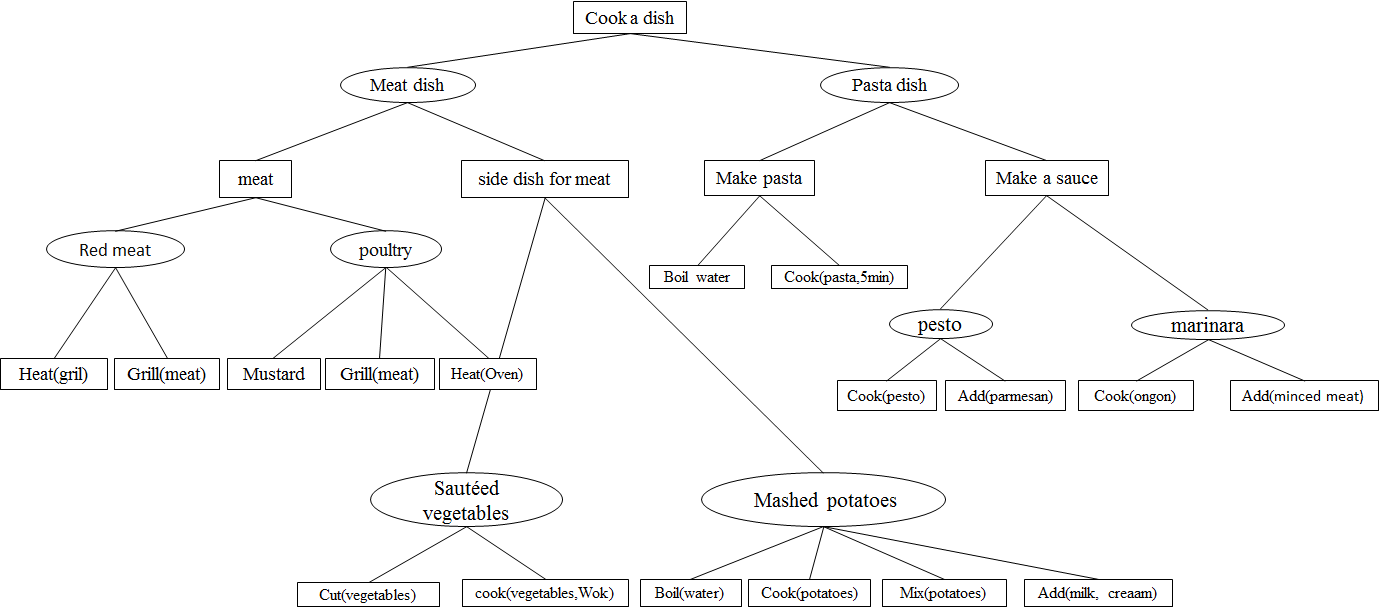
\includegraphics[width=\textwidth]{Pictures/cooking.png}
 	\caption{\label{Cooking model example} Cooking model example}
 \end{figure}
 

In addition, reactive HTNs take the position of using no planning process to detects the future state. Instead, the HTN plans only for the next task to be executed  based only on the current observable state. HTNs use procedural definition of the domain knowledge that can offer no reasoning and  uses an optimistic valuation of the conditions . This execution approach can lead the HTN to a state where no decomposition or execution are possible, this state is then called dead end. In such case, we say that the HTN executor faces a breakdown.Because of the procedural definition of the domain knowledge and the reactive formalism of the HTN, this later is unable to backtrack in order to find another way to achieve the goal task.
Therefore, the HTN can no longer continue its execution and the goal is impossible to achieve.

For example, lets the HTN describing the move\&paint task execution presented in Figure \ref{break example}. The HTN starts the decomposition from the top level goal and at each step it monitors the conditions of each task. Once it attempts primitive tasks, the execution in the real world starts. the HTN starts by executing the pickup(Object) task, by first evaluating its preconditions, after the execution of the task, the HTN evaluates its  postcondition. Arriving to the execution of the Walk task,  the world changes in unexpected way; assume that the wind blows and the door is now blocked.Thus, the preconditions of the Walk(room1, room2, door1) task (i.e IsOpen(Door)) are no longer valid. the HTN execution is then blocked and a breakdown is then detected.
 \begin{figure}[h]
 	\centering
 	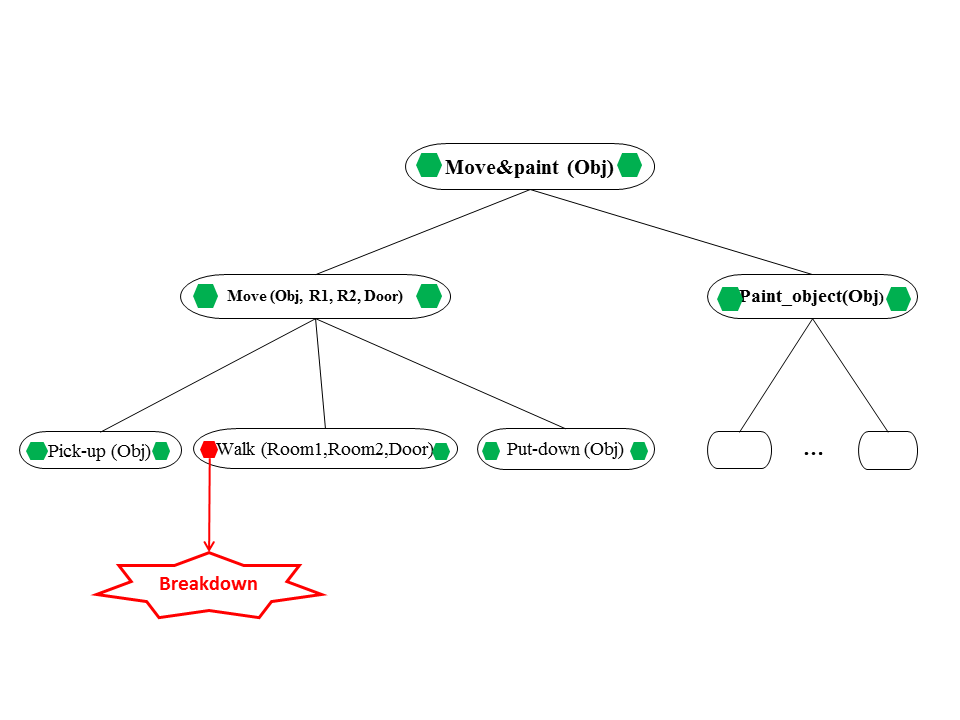
\includegraphics[width=\textwidth]{Pictures/break.png}
 	\caption{\label{break example} Breakdown situation in the move\&paint example}
 \end{figure}
 
 \section{Conclusion}
This chapter presented the background of our work.First, we presented and discussed the existing methods in the field of planning, from linear planning to hierarchical planning. Then we defined  the addressed problem which concerns breakdowns especially in reactive HTN, and the necessity of recovering from breakdowns taking in account the incompleteness of reactive HTN's knowledge domain.

In the next chapter (chapter3), we will put forward the existing approaches to recover from breakdowns and discuss their utility in the addressed problem. Next, we will present in chapter 4 the proposed solution to recover from breakdowns in reactive HTN with incomplete models and details the architecture of the plan recover system. 
 